\documentclass[problem]{mcs}

\begin{pcomments}
  \pcomment{PS_3color_SAT}
  \pcomment{by ARM October 25, 2011, edited with new figure 4/4/12}
\end{pcomments}

\pkeywords{
SAT
logical_formula
propositional_logic
logic
proposition
negation
coloring
}

%%%%%%%%%%%%%%%%%%%%%%%%%%%%%%%%%%%%%%%%%%%%%%%%%%%%%%%%%%%%%%%%%%%%%
% Problem starts here
%%%%%%%%%%%%%%%%%%%%%%%%%%%%%%%%%%%%%%%%%%%%%%%%%%%%%%%%%%%%%%%%%%%%%

\begin{problem}
Let $G$ be the $11$- vertex graph of Figure~\ref{fig:coloring_no_triangles}. This problem shows that its chromatic number is 4, even though it has no triangles.

\inhandout{\newpage}
\begin{figure}\inbook{[hb]}
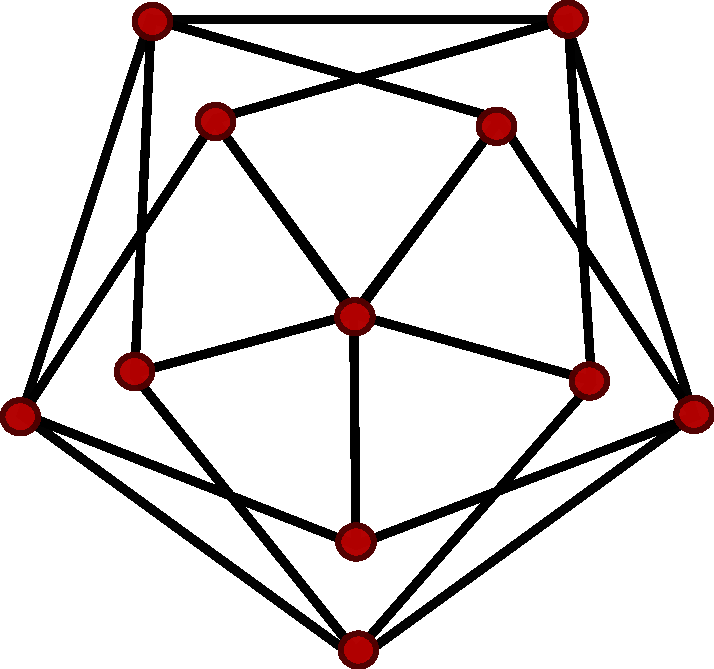
\includegraphics[width=2in]{../figures/drafts/coloring_no_triangles}
\caption{Graph with 11 vertices and no triangles}
\label{fig:coloring_no_triangles}
\end{figure}



\bparts

\ppart Show that $G$ is 4-colorable.

\begin{solution}
  Figure \ref{fig:coloring_no_triangles_solution} shows a valid coloring.
\begin{figure}\inbook{[h]}
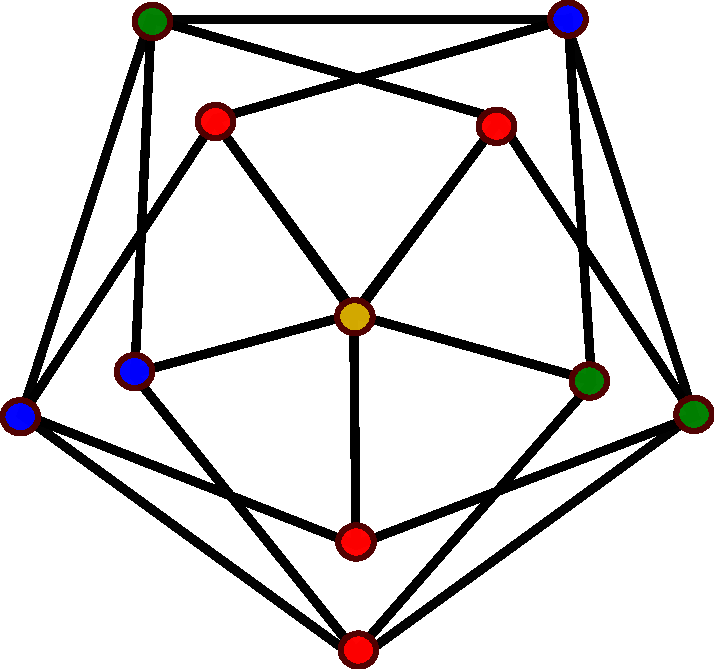
\includegraphics[width=2in]{../figures/drafts/coloring_no_triangles_solution}
\caption{Coloring using 4 colors}
\label{fig:coloring_no_triangles_solution}
\end{figure}
\end{solution}

\ppart\label{fgateforNOTOR}Show that $G$ can't be colored with $3$ colors. 


\begin{solution}
   Assume by contradiction that there is one coloring using only 3 colors: red, blue and green. First, consider only the outer pentagon of the graph. Notice  that it is impossible to color it using only two colors. Thus, we can assume that the outer pentagon is colored as shown in the left of Figure \ref{fig:coloring_no_triangles_solution2}.

  Now, observe that there are three points in the interior whose color is determined, as shown in the right of Figure \ref{fig:coloring_no_triangles_solution2}. Note that the point in the center has neighbors with all three colors so it is impossible to color it.


\begin{figure}\inbook{[h]}
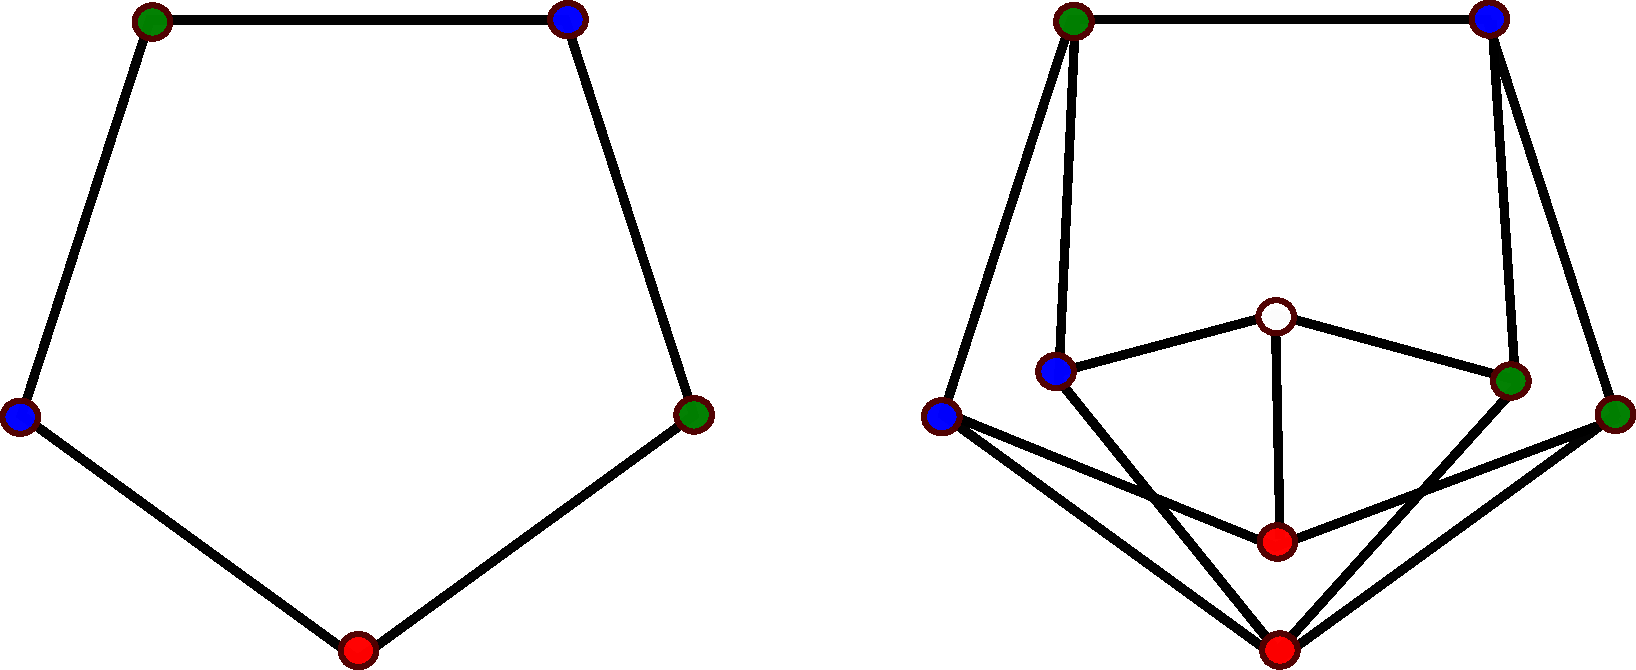
\includegraphics[width=4in]{../figures/drafts/coloring_no_triangles_solution2}
\caption{Structure of a valid coloring with 3 colors.}
\label{fig:coloring_no_triangles_solution2}
\end{figure}
\end{solution}
\eparts

\end{problem}

%%%%%%%%%%%%%%%%%%%%%%%%%%%%%%%%%%%%%%%%%%%%%%%%%%%%%%%%%%%%%%%%%%%%%
% Problem ends here
%%%%%%%%%%%%%%%%%%%%%%%%%%%%%%%%%%%%%%%%%%%%%%%%%%%%%%%%%%%%%%%%%%%%%

\endinput
